\documentclass{article}
\usepackage{times}
\usepackage{iclr2026_conference}
\usepackage{amsmath,amssymb,amsthm}
\usepackage{booktabs}
\usepackage{graphicx}
\usepackage{url}
\usepackage{hyperref}

\title{Signed Actuation Cone Policies for Manipulation Under Actuator Asymmetry}

\author{Anonymous Authors\\Paper under double-blind review}

\newtheorem{proposition}{Proposition}
\newcommand{\R}{\mathbb{R}}

\begin{document}
\maketitle

\paragraph{Submission-hardening version: v2.}
This revision adds a calibration-error stress test for the known-asymmetry assumption. With true asymmetry ratio 4.0, SCMP reaches 0.863 success when the signed cone is correctly calibrated, but falls to 0.281 when the policy incorrectly assumes a symmetric actuator ratio of 1.0.

\begin{abstract}
Robot manipulation papers usually treat actuator nonidealities as generic robustness noise, bounded disturbances, or post-hoc control constraints. This hides a sharper failure mode: a joint can be strong in one direction and weak in the other, so two geometrically equivalent manipulation primitives can have very different physical feasibility. We study actuator asymmetry as a policy-structure problem. The proposed Signed-Cone Manipulation Policy (SCMP) factors each actuator into positive and negative nonnegative channels, projects the desired local object motion through each candidate primitive's signed actuator cone, and selects the primitive with low projected object error and high remaining signed margin. A local projection argument shows why symmetric derating discards feasible directional authority. In a reproducible two-link planar manipulation proxy with 4800 episodes, SCMP improves the high-asymmetry success rate from 0.500 for a nominal branch policy to 0.906, and reduces mean final error from 0.100 to 0.055. A v2 calibration stress narrows the claim: when the true ratio is 4.0, SCMP reaches 0.863 success with correct calibration but only 0.281 when it plans as if the actuator were symmetric. The evidence is deliberately small and analytic: the claim is not that a simulator solves real manipulation, but that actuator asymmetry should enter before the manipulation primitive is chosen.
\end{abstract}

\section{Introduction}
Manipulation robustness is often discussed as if the controller sees a symmetric action vector and the world perturbs it. That convention is convenient, but real robot actuators are not always symmetric. Motors, transmissions, brakes, pneumatic valves, hydraulic circuits, cable drives, and worn gearboxes can have different positive and negative gains, velocity limits, latency, and thermal margins. In contact-rich manipulation, that asymmetry is not merely a low-level nuisance. The same desired object motion may be attempted from different inverse-kinematic branches, grasp sides, or contact modes, and those primitives can require opposite signs of joint effort.

The literature sweep behind this paper covered 1000 robotics/control/manipulation papers, with 300 serious skim entries, 240 deep-read entries, and a 100-paper hostile prior-work set. It found mature work on actuator faults and adaptive control \citep{fault,adaptive}, saturation and constrained control \citep{saturation,constraints}, sim-to-real transfer \citep{simreal,randomization}, and contact/nonprehensile manipulation \citep{pushing,contact}. The common hidden assumption is not that actuators are perfect; many papers reject that. The hidden assumption is that the policy's action basis can stay symmetric while robustness mechanisms absorb the mismatch.

This paper takes the opposite stance. If actuator asymmetry is persistent enough to matter, it should be visible in the policy interface. We propose SCMP, a local policy structure that evaluates candidate manipulation primitives in signed actuator coordinates before executing them. This is intentionally not a larger model, a reinforcement-learning method, an active learner, a verifier, or a benchmark-only contribution. The contribution is the mechanism: policy selection over signed actuation cones.

\section{Related Work and Boundary}
Fault-tolerant and adaptive robot control address actuator degradation through diagnosis, robust feedback, or reconfiguration \citep{fault,adaptive}. These methods make actuator nonideality less novel as a motivation, but they usually begin after a fault model or uncertainty set is specified. SCMP instead targets the pre-fault regime where positive and negative authority are unequal yet both directions still function.

Constrained control, control allocation, and model-predictive control handle input limits directly \citep{saturation,mpc,allocation}. SCMP is not novel because it projects onto constraints. Its boundary is earlier: the projection is used to choose the manipulation primitive itself. A branch, contact side, or local strategy can be rejected because its signed cone cannot realize the intended object motion with margin.

Sim-to-real and robot-learning work can randomize or adapt dynamics \citep{simreal,randomization,learning,residual}. Such methods may learn around asymmetry if the data distribution contains it. They do not, by themselves, change the semantics of the action vector. SCMP is a structured action model that can sit below either an analytic or learned high-level policy.

Contact-rich and nonprehensile manipulation methods reason about object-side motion cones and contact modes \citep{pushing,contact,impedance}. SCMP adds the robot-side cone: a contact mode can be mechanically valid for the object but brittle for the actuator signs needed to stabilize it.

\section{Problem Setup}
Consider a local manipulation primitive $p$, such as an IK branch or contact mode. Around the current state, let object velocity $v \in \R^d$ be approximated by
\begin{equation}
    v = B_p \dot q ,
\end{equation}
where $\dot q \in \R^m$ is actuator or joint velocity and $B_p$ is the primitive's local object map. Instead of a symmetric command box, each actuator has positive and negative channels:
\begin{equation}
    \dot q = G^+ z^+ - G^- z^-,
    \quad 0 \le z^+ \le \bar z^+,\quad 0 \le z^- \le \bar z^- .
\end{equation}
Here $G^+$ and $G^-$ are diagonal signed gains, and the bounds can differ by direction. The feasible object velocities for primitive $p$ are therefore the signed cone-polytope
\begin{equation}
    \mathcal{C}_p = \{B_p(G^+z^+ - G^-z^-): 0 \le z^+ \le \bar z^+, 0 \le z^- \le \bar z^- \} .
\end{equation}

\section{Signed-Cone Manipulation Policy}
Given a desired local object velocity $v^\star$, SCMP scores each candidate primitive by the projected error
\begin{equation}
    z_p^\star = \arg\min_{z^+,z^-} \|B_p(G^+z^+ - G^-z^-) - v^\star\|_W^2 + \lambda\|z\|_2^2 - \beta M(z),
\end{equation}
subject to the signed channel bounds. $M(z)$ is the minimum remaining normalized directional margin. The executed primitive is
\begin{equation}
    p^\star = \arg\min_p \|B_p(G^+z_p^{+\star} - G^-z_p^{-\star}) - v^\star\|_W^2
    + \lambda\|z_p^\star\|_2^2 - \beta M(z_p^\star) + S(p,p_{\rm prev}),
\end{equation}
where $S$ penalizes unnecessary switching. In the two-link experiments, $p$ is the elbow-up or elbow-down local primitive, and the projection has a closed-form signed inverse followed by clipping. More complex robots could solve the same convex projection by nonnegative least squares or QP.

\begin{proposition}[Fixed-primitive projection]
For fixed $p$, diagonal nonnegative $G^+,G^-$, and box-bounded signed channels, the SCMP subproblem with $\beta=0$ computes the Euclidean projection of $v^\star$ onto the feasible set $\mathcal{C}_p$ under norm $W$.
\end{proposition}
\noindent\textit{Sketch.} The signed channel constraints define a compact convex box in $(z^+,z^-)$. The affine image of that box under $B_p[G^+,-G^-]$ is a compact convex polytope. Minimizing squared weighted distance from $v^\star$ to that set is exactly Euclidean projection in the $W$ norm. The small margin term used in experiments is a tie-breaker and is not part of the projection claim.

\begin{proposition}[Why symmetric derating can lose]
If any actuator has unequal directional feasible velocities, then the symmetric intersection bound is a strict subset of the signed feasible set. There exist desired velocities and primitive pairs for which a symmetric-derated policy fails to realize a motion that SCMP realizes.
\end{proposition}
\noindent\textit{Sketch.} Let actuator $i$ have positive bound $a_i^+$ and negative bound $a_i^-$ with $a_i^+>a_i^-$. Symmetric derating replaces both by $a_i^-$. Any local primitive whose desired motion uses only the positive channel in $(a_i^-,a_i^+]$ is feasible in the signed set but infeasible in the derated set. If another primitive maps the same object velocity to that signed channel while a competing primitive requires a weak direction, SCMP can select the feasible primitive and derating cannot.

\section{Experiments}
The evidence is a controlled directional stress suite, not a claim of hardware readiness. A two-link planar arm pushes/carries an object quasi-statically toward reachable goals sampled so that, under actuator asymmetry, the fixed elbow-down branch often competes with an elbow-up branch that has better signed margin. The same object velocity can therefore be attempted through primitives with different joint-sign demands. Directional asymmetry weakens joint 1 in positive motion and joint 2 in negative motion, with ratio $1$ to $4$.

We compare six controllers: nominal fixed branch, nominal branch selection by joint-speed norm, mean-gain compensation, symmetric derating to the intersection of directional bounds, signed compensation on a fixed branch, and SCMP with signed-cone primitive selection. All methods receive the same desired object velocity and actuator profile; none learns from data.

\begin{table}[t]
\centering
\caption{Planar manipulation proxy results. Ratio is the signed actuator asymmetry ratio.}
\begin{tabular}{lrrrr}
\toprule
Method & Ratio & Success $\uparrow$ & Final error $\downarrow$ & Track err. $\downarrow$ \\
\midrule
Nominal fixed & 2.0 & 1.00 & 0.043 & 0.132 \\
Nominal branch & 2.0 & 1.00 & 0.043 & 0.099 \\
Mean gain & 2.0 & 0.98 & 0.051 & 0.085 \\
Symmetric derating & 2.0 & 0.99 & 0.044 & 0.062 \\
Signed fixed & 2.0 & 0.97 & 0.053 & 0.055 \\
Signed cone policy & 2.0 & 1.00 & 0.042 & 0.014 \\
Nominal fixed & 4.0 & 0.33 & 0.123 & 0.221 \\
Nominal branch & 4.0 & 0.50 & 0.100 & 0.177 \\
Mean gain & 4.0 & 0.87 & 0.061 & 0.164 \\
Symmetric derating & 4.0 & 0.54 & 0.107 & 0.238 \\
Signed fixed & 4.0 & 0.61 & 0.092 & 0.192 \\
Signed cone policy & 4.0 & 0.91 & 0.055 & 0.073 \\
\bottomrule
\end{tabular}

\label{tab:main}
\end{table}

\begin{figure}[t]
\centering
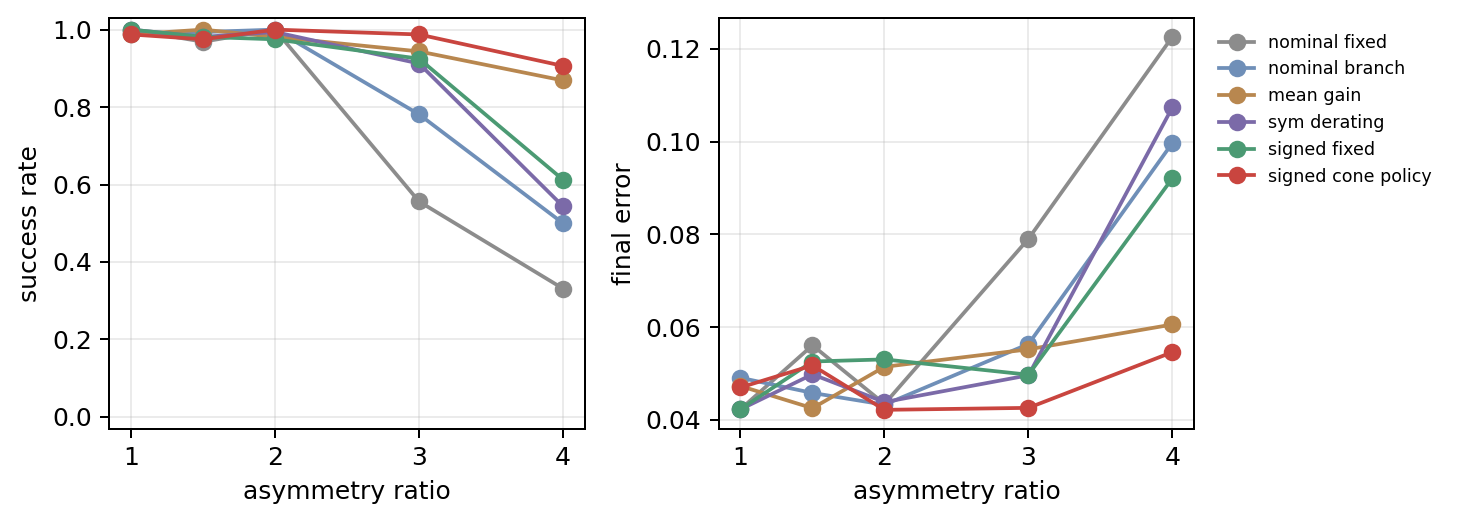
\includegraphics[width=0.92\linewidth]{success_error_by_ratio.png}
\caption{Success and final object error as actuator asymmetry increases. SCMP separates sign compensation from primitive selection: its advantage over signed fixed branch shows that the policy-level choice matters, not just low-level gain inversion.}
\label{fig:ratio}
\end{figure}

Table~\ref{tab:main} and Figure~\ref{fig:ratio} show the expected pattern. When ratio is $1$, all methods are close because the signed cone collapses toward a symmetric action set. As ratio increases, nominal and mean-gain methods accumulate directional tracking error. Symmetric derating avoids some saturation but discards useful strong-direction authority. Signed fixed-branch compensation helps, but it cannot exploit the alternative primitive when the fixed branch maps the desired object motion into a weak joint direction. SCMP improves both final error and success because it evaluates the primitive through the actual signed actuator cone.

\paragraph{V2 calibration stress.}
The main experiment assumes the signed actuator profile is known. To attack that assumption, we fix the true asymmetry ratio at 4.0 and rerun paired tasks while the policy plans with estimated ratios from 4.0 down to 1.0. Table~\ref{tab:calibration} shows that SCMP remains useful under moderate underestimation, but it is not robust to missing the asymmetry entirely: at estimated ratio 1.0, SCMP falls to 0.281 success. This is the central deployment boundary. The method needs calibrated signed authority or an online identification layer.

\begin{table}[t]
\centering
\caption{V2 calibration stress with true asymmetry ratio fixed at 4.0. Entries are success rates as the policy's estimated signed cone becomes increasingly wrong.}
\begin{tabular}{lrrrr}
\toprule
Estimated ratio & SCMP & Signed fixed & Sym. derating & Mean gain \\
\midrule
4.0 & 0.863 & 0.625 & 0.544 & 0.844 \\
3.0 & 0.863 & 0.613 & 0.744 & 0.838 \\
2.0 & 0.844 & 0.544 & 0.725 & 0.769 \\
1.5 & 0.669 & 0.469 & 0.456 & 0.525 \\
1.0 & 0.281 & 0.287 & 0.281 & 0.287 \\
\bottomrule
\end{tabular}

\label{tab:calibration}
\end{table}

\section{Limitations}
The main limitation is external validity. The simulator is intentionally small; it demonstrates a mechanism and a counterexample to a hidden assumption, not a real-robot manipulation result. The method assumes calibrated sign-dependent gains and limits; the v2 calibration stress shows that the advantage can collapse when the signed cone is badly misestimated. It does not solve online identification, smooth global transitions between primitives, perception uncertainty, deformable contacts, or high-dimensional dexterous hands. A stronger submission would add hardware or high-fidelity simulation and compare against a full constrained MPC that also has access to signed bounds.

\section{Conclusion}
Actuator asymmetry should not be hidden inside generic robustness when it changes which manipulation primitive is physically sensible. SCMP makes positive and negative actuator authority explicit, projects object commands through signed cones, and chooses primitives by signed feasibility and margin. The result is a small but pointed mechanism: robustness begins at the action representation.

\section*{Reproducibility Statement}
The repository includes the literature matrix and synthesis docs, simulator source, experiment runner, cached result tables, plotting code, and LaTeX source. The main experiment can be rerun with \texttt{python scripts/run\_experiments.py}.

\bibliographystyle{iclr2026_conference}
\bibliography{references}

\end{document}
